\section{ELR validation including the four-fermion parameter space}
\label{sec:9dvalidation}
Fifty test-samples with all nine coefficients varying are separated for further validation of the full parameter space. Reasonable modeling is found in all regions. 
\begin{figure}[h!]
  \begin{minipage}[b]{0.495\linewidth}
    \centering
    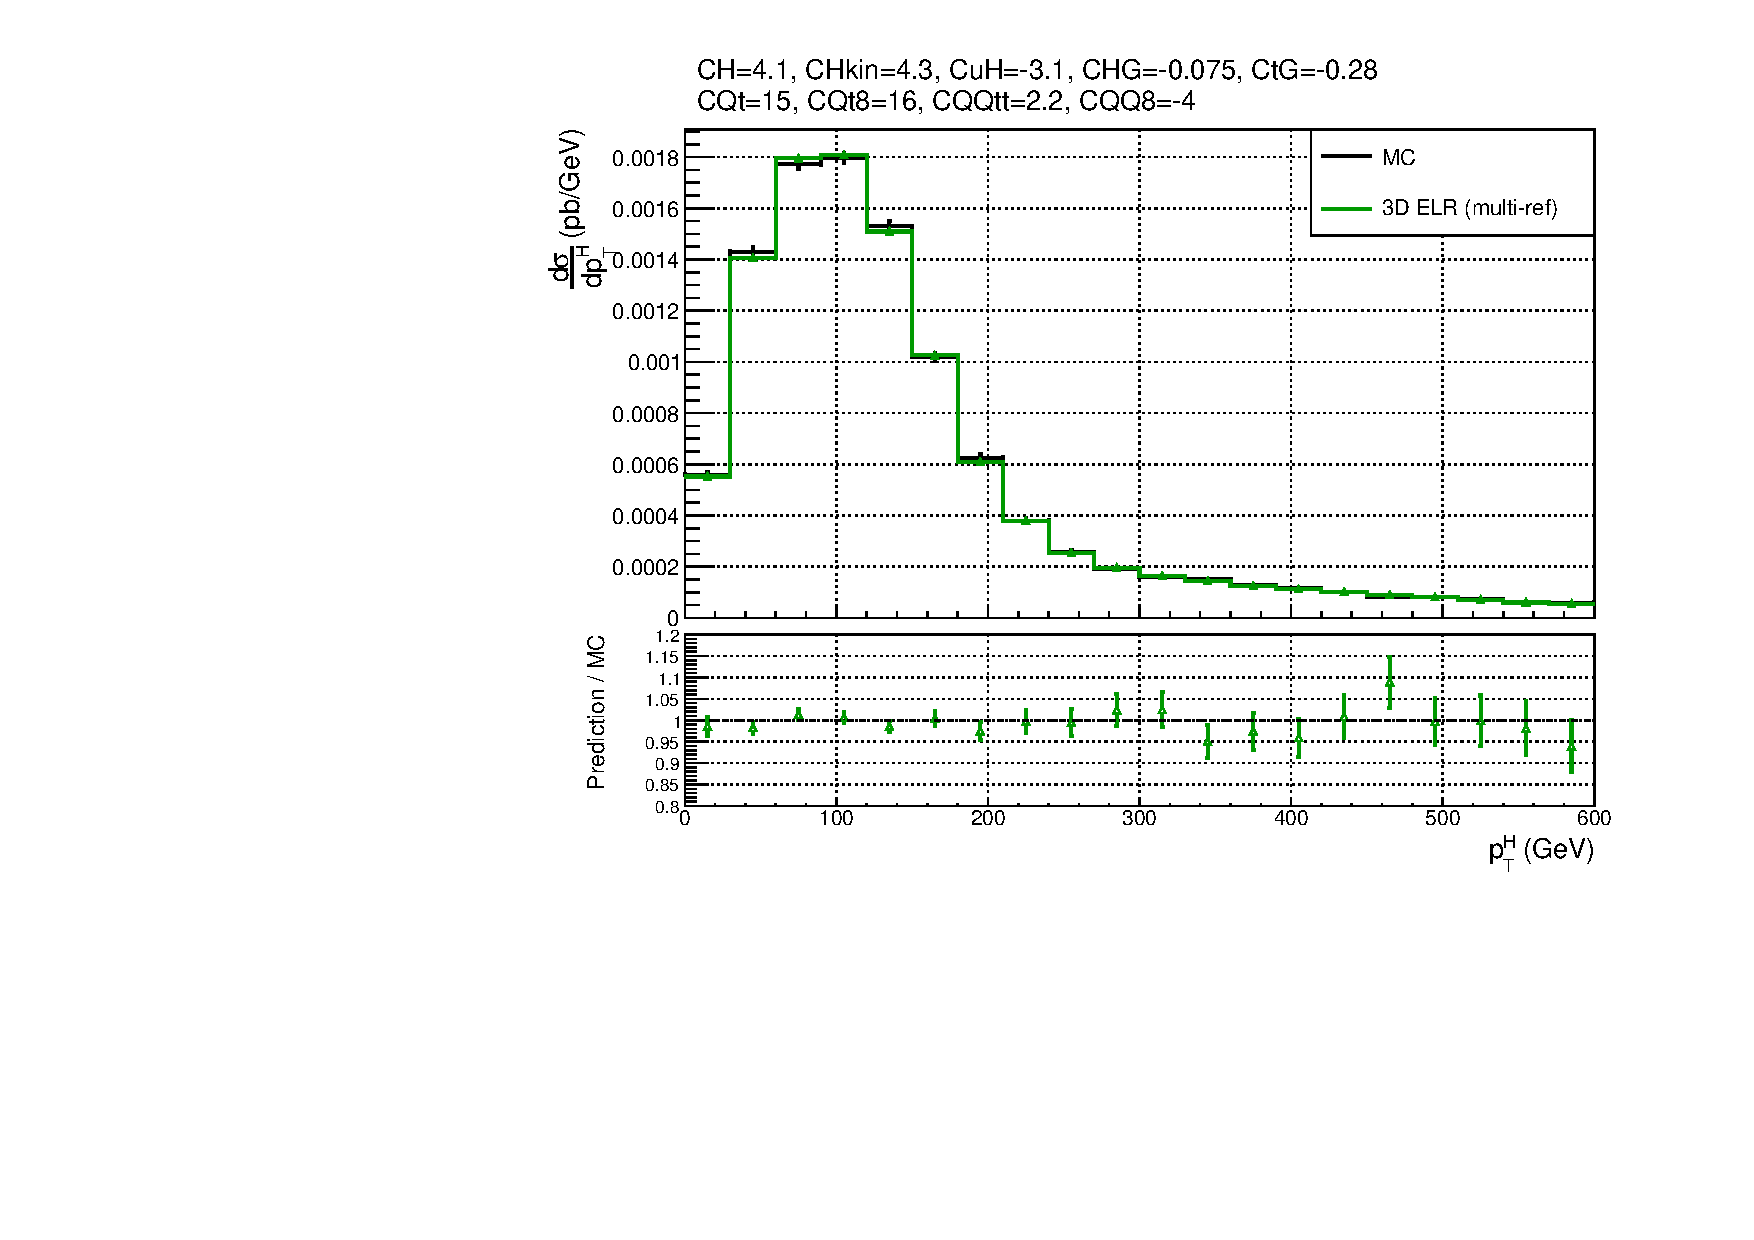
\includegraphics[width=\linewidth]{plots/pth_3d_multiref_(48)_CH_4.13477_CHbox_4.34845_CuH_-3.1115_CHG_-0.0753981_CtG_-0.282248_CQt_15.0718_CQt8_15.8966_CQQtt_2.22505_CQQ8_-3.9732.pdf}
  \end{minipage}
  \hfill
  \begin{minipage}[b]{0.495\linewidth}
    \centering
    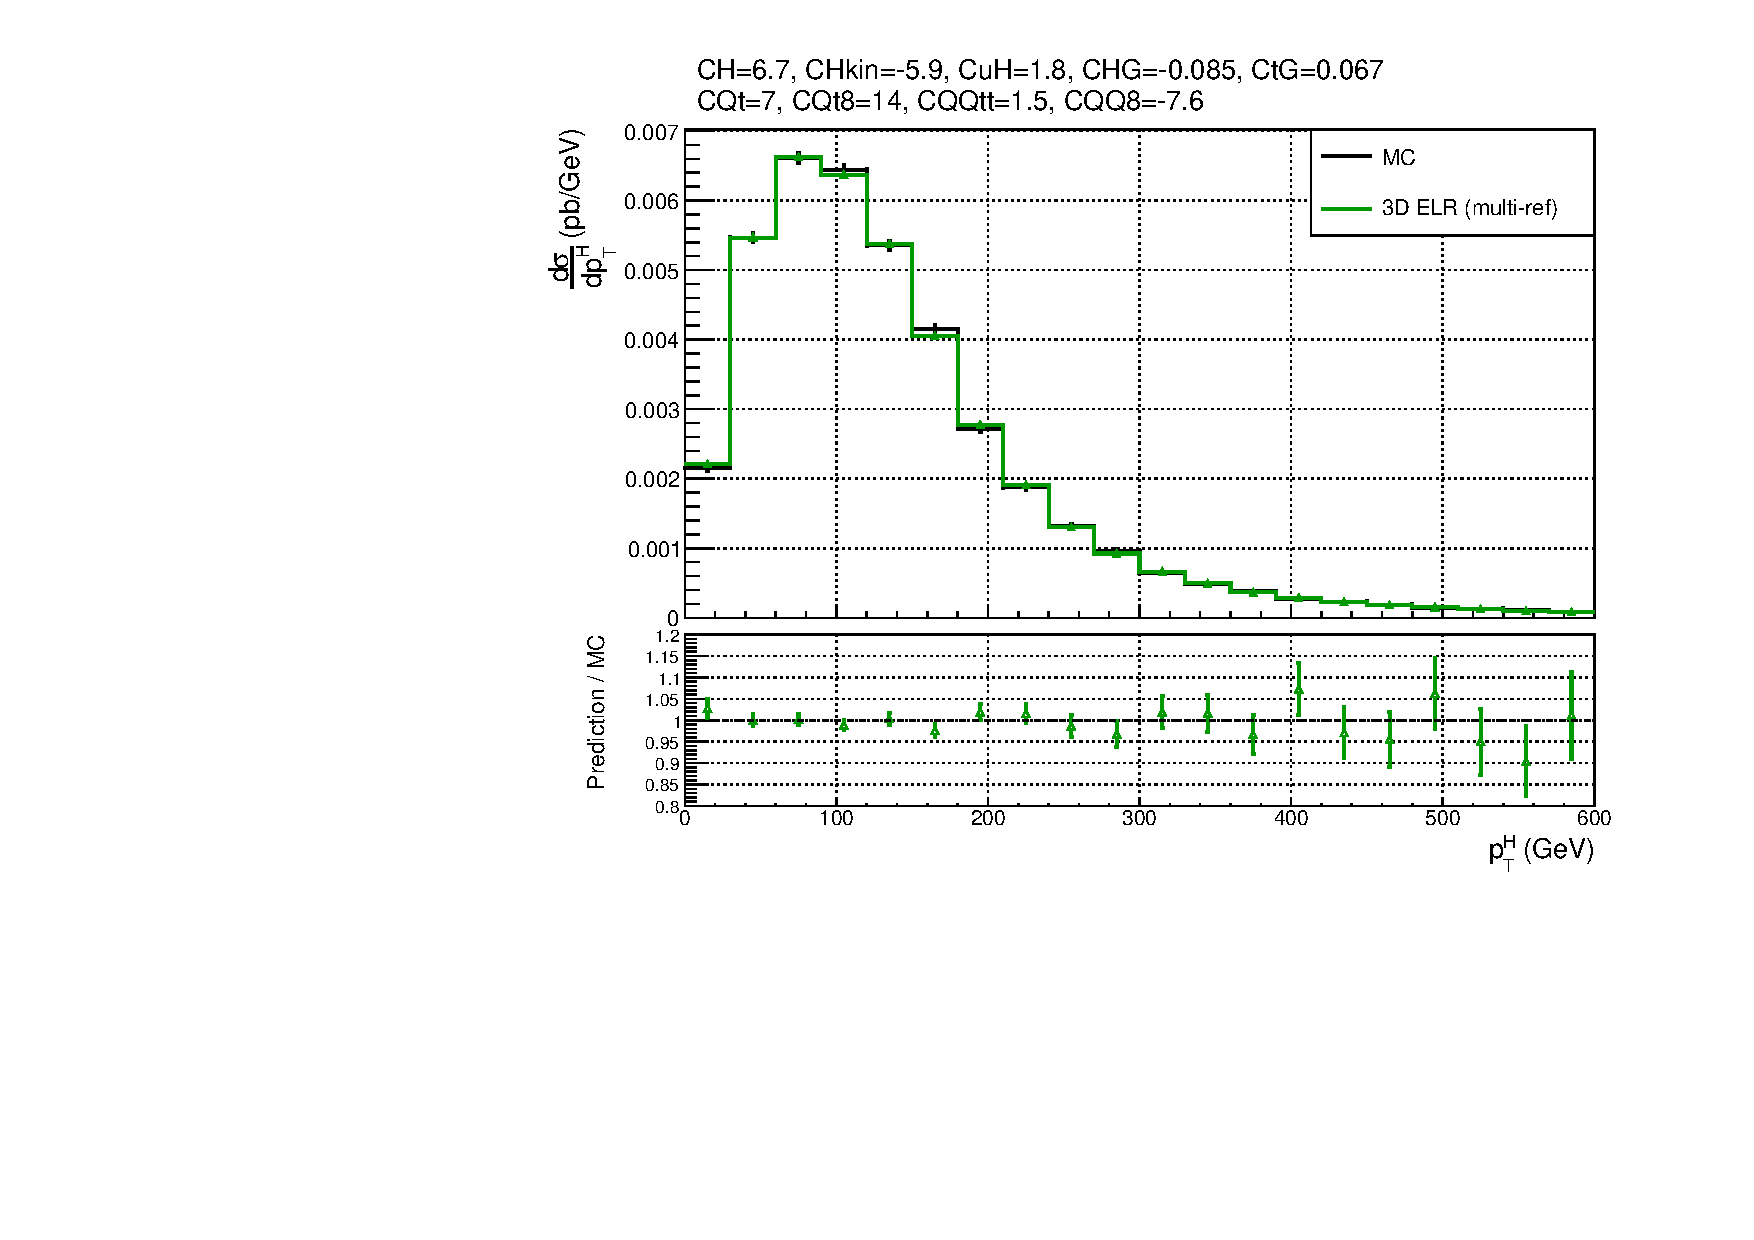
\includegraphics[width=\linewidth]{plots/pth_3d_multiref_(49)_CH_6.67517_CHbox_-5.89157_CuH_1.83813_CHG_-0.0845237_CtG_0.0674596_CQt_7.02121_CQt8_13.5041_CQQtt_1.45086_CQQ8_-7.61857.pdf}
  \end{minipage}
  \caption{Higgs transverse momenta distributions for some of the 9D test-samples generated at $\sqrt{s}=13.6$ TeV.}
  \label{fig:pth3}
\end{figure}
\begin{figure}[h!]
    \centering    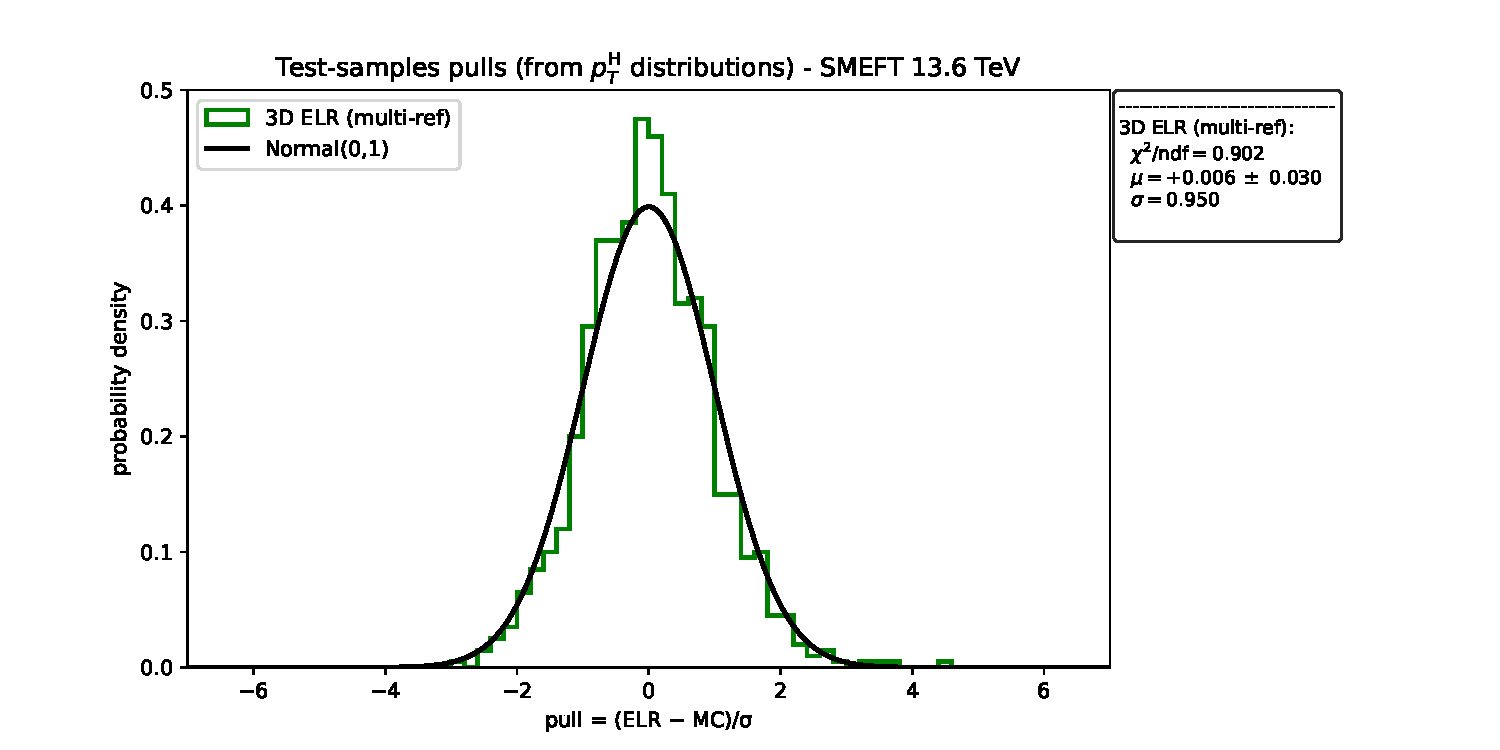
\includegraphics[width=1\linewidth]{plots/stats3.pdf}
    \caption{Pulls and statistical parameters obtained from $p^\text{H}_T$ bins in SMEFT with test-samples varying all the nine coefficients.}
    \label{fig:stats3}
\end{figure}
%\textcolor{red}{TODO: list the 50 held-out SMEFT samples (25 from the 2D grids and 25 from the 9D Gaussian) with their Wilson coefficient values.}
